%! Author = mariuszindel
%! Date = 25.01.21

\section{Block Code}


\subsection{Hammingdistanz $h$}
\begin{itemize}
    \item sicher korrigierbarer Fehler, wenn
    \item $m$ = Nachrichtenstellen
    \item $k$ = Kontrollstellen
\end{itemize}
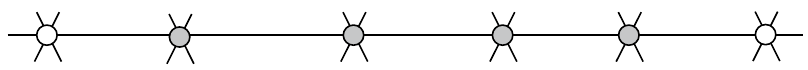
\includegraphics[width=\linewidth]{graphic/extern-reto/Hammingdistanz.png}
Jeder Knoten ist ein \textcolor{red}{Codewort}!\\
Sichere Erkennung von 4 Fehlern $\rightarrow$ Hammingdistanz = 5\\\\

\subsubsection{Anzahl gültige Codeworte}
\colorbox{lightlightgrey}{$2^m$}

\subsubsection{Anzahl der möglichen Codeworte}
\colorbox{lightlightgrey}{$2^{m+k}$}

\subsubsection{Sicher kkorrigierbarer Fehler}
$h$ \textcolor{red}{ungerade}: \colorbox{lightlightgrey}{$e = \frac{h - 1}{2}$}\hspace{3cm}$h$ \textcolor{red}{gerade}: \colorbox{lightlightgrey}{$e = \frac{h - 2}{2}$}

\subsubsection{Dichtgepackt}
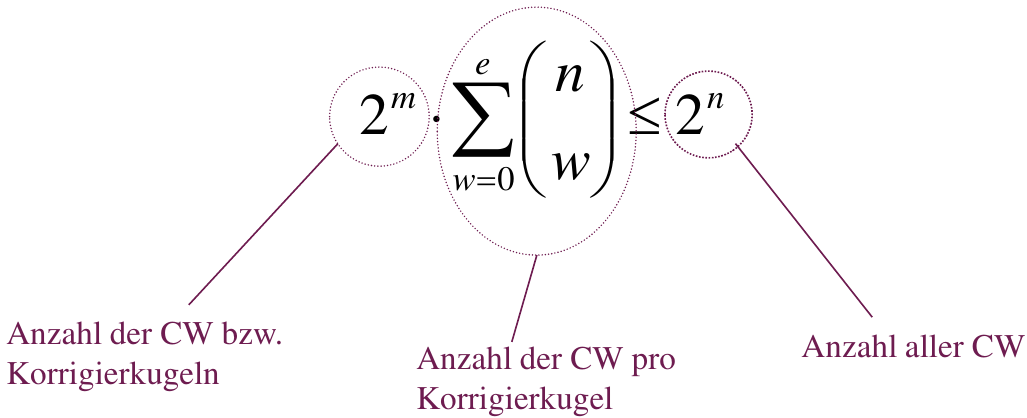
\includegraphics[width=\linewidth]{graphic/extern-reto/Dichtgepackt.png}\\
Wenn linker Teil = rechter Teil, so ist der Coderaum \textcolor{red}{Dichtgepackt}


\subsection{Prüfmatrix eines Hammingcodes}

\subsubsection{Anzahl Kontrollstellen $k$}
Bei Hammingcodes markiert die Einheitsmatrix in der Prüfmatrix die Anzahl der Kontrollstellen \colorbox{lightlightgrey}{$k = $ Spalten der Einheitsmatrix}

\subsubsection{gueltige Codeworte}
$m$ = Anzahl Spalten der Prüfmatrix bis zur Einheitsmatrix\\
\colorbox{lightlightgrey}{gueltige Codeworte = $2^m$}


\vfill
$$
\columnbreak